%%%%%%%%%%%%%%%%%%%%%%%%%%%%%%%%%%%%%%%%%%%%%%%%%%%%%%%%%%%%%%%%%%%%%%%%%%%%%%%%
% AMS Beamer series / Bologna FC / Template
% Andrea Omicini
% Alma Mater Studiorum - Università di Bologna
% mailto:andrea.omicini@unibo.it
%%%%%%%%%%%%%%%%%%%%%%%%%%%%%%%%%%%%%%%%%%%%%%%%%%%%%%%%%%%%%%%%%%%%%%%%%%%%%%%%
%\documentclass[handout]{beamer}\mode<handout>{\usetheme{default}}
%
\documentclass[presentation, 9pt,169]{beamer}\mode<presentation>{\usetheme{AMSBolognaFC}}
%\documentclass[handout]{beamer}\mode<handout>{\usetheme{AMSBolognaFC}}
%%%%%%%%%%%%%%%%%%%%%%%%%%%%%%%%%%%%%%%%%%%%%%%%%%%%%%%%%%%%%%%%%%%%%%%%%%%%%%%%
\usepackage[T1]{fontenc}
\usepackage{wasysym}
\usepackage{amsmath,blkarray}
\usepackage{soul}
\usepackage[minted,most]{tcolorbox}
\usepackage{centernot}
\usepackage{fontawesome}
\usepackage{fancyvrb}
\usepackage{minted}
\usepackage{hyperref}
\usepackage{multicol}
\usepackage{tcolorbox}
\usepackage{etoolbox}
\BeforeBeginEnvironment{minted}{\begin{tcolorbox}}%
\AfterEndEnvironment{minted}{\end{tcolorbox}}%
\setminted[scala]{fontsize=\small,baselinestretch=1,obeytabs=true, tabsize=2}
\setminted[yaml]{fontsize=\large,frame=lines,linenos,baselinestretch=1,obeytabs=true, tabsize=2}
\usepackage[ddmmyyyy]{datetime}
\setminted{fontsize=\footnotesize}
\renewcommand{\dateseparator}{}
%\renewcommand{\thefootnote}{\fnsymbol{footnote}}
\newcommand{\version}{1}

\usepackage[
	%backend=biber,
	backend=bibtex,
%	citestyle=authoryear-icomp,
%	maxcitenames=1,
	style=alphabetic]{biblatex}

	\makeatletter

%\addbibresource{biblio.bib}

\bibliography{biblio}

\newcommand\extrafootertext[1]{%
    \bgroup
    \renewcommand\thefootnote{\fnsymbol{footnote}}%
    \renewcommand\thempfootnote{\fnsymbol{mpfootnote}}%
    \footnotetext[0]{#1}%
    \egroup
}

\newcommand{\citeinslide}[1]{\cite{#1}\extrafootertext{\scriptsize\cite{#1} \fullcite{#1}}}


%%%%%%%%%%%%%%%%%%%%%%%%%%%%%%%%%%%%%%%%%%%%%%%%%%%%%%%%%%%%%%%%%%%%%%%%%%%%%%%%
\title[A Soft-Eng Approach for CPSWs!]
{A Language-based Software Engineering Approach for Cyber-Physical Swarms}
%
%
\author[\sspeaker{G.Aguzzi}]
{\speaker{Gianluca Aguzzi} \href{mailto:gianluca.aguzzi@unibo.it}{gianluca.aguzzi@unibo.it} \\
\textbf{Supervisor:} \speaker{Mirko Viroli} \href{mailto:mirko.viroli@unibo.it}{mirko.viroli@unibo.it}}
%
\institute[DISI, Univ.\ Bologna]
{%Dipartimento di Informatica -- Scienza e Ingegneria (DISI)\\
\textsc{Alma Mater Studiorum} -- Universit{\`a} di Bologna \\[0.1cm]
\textbf{PhD defense}\\[0.15cm]
}
%
\renewcommand{\dateseparator}{/}
\date[\today]{\today}
%
\AtBeginSubsection[]
{
  \begin{frame}
  \frametitle{Contents}
  \tableofcontents[currentsubsection, 
	sectionstyle=show/shaded, 
	subsectionstyle=show/shaded]
  \end{frame}
}
\AtBeginSection[]
{
  \begin{frame}
  \frametitle{Contents}
  \tableofcontents[currentsubsection, 
	sectionstyle=show/shaded, 
	subsectionstyle=show/shaded]
  \end{frame}
}
%%%%%%%%%%%%%%%%%%%%%%%%%%%%%%%%%%%%%%%%%%%%%%%%%%%%%%%%%%%%%%%%%%%%%%%%%%%%%%%%

\lstdefinelanguage{scala}{
  keywords={abstract,case,catch,class,def,%
    do,else,extends,false,final,finally,%
    for,if,implicit,import,match,mixin,%
    new,null,object,override,package,%
    private,protected,requires,return,sealed,%
    super,this,throw,trait,true,try,lazy,%
    type,val,var,while,with,yield,forSome},
  otherkeywords={=>,<-,<\%,<:,>:,\#},
  sensitive=true,
  morecomment=[l]{//},
  morecomment=[n]{/*}{*/},
  morestring=[b]",
  morestring=[b]',
  morestring=[b]""",
  basicstyle=\lst@ifdisplaystyle\footnotesize\fi\ttfamily,
  emphstyle=\bfseries
}
\definecolor{ddarkgreen}{rgb}{0,0.5,0}
\lstdefinelanguage{scafi}{frame=single,basewidth=0.5em,language={scala},
keywordstyle=\color{blue}\textbf, commentstyle=\color{ddarkgreen},
keywordstyle=[2]\color{red}\textbf, keywords=[2]{rep,nbr,foldhood,foldhoodPlus,aggregate,branch,spawn},
keywordstyle=[3]\color{gray}, keywords=[3]{Me,AroundMe,Everywhere,Forever}, %,@@,@@@
keywordstyle=[4]\color{red}\textbf, keywords=[4]{in,out,rd},
keywordstyle=[5]\color{violet}, keywords=[5]{evolve,when,andNext,workflow,C,gossip},
keywordstyle=[6]\color{orange}, keywords=[6]{Available,Serving,Done,Waiting,Removing}}

\newcommand{\hsplit}[2]{
\begin{minipage}{0.48\textwidth}
#1
\end{minipage}
\hfill
\begin{minipage}{0.48\textwidth}
#2
\end{minipage}
}
\newcommand{\hsplits}[4]{
\begin{minipage}{#1\textwidth}
#3
\end{minipage}
\hfill
\begin{minipage}{#2\textwidth}
#4
\end{minipage}
}

\newcommand{\lbl}[1]{\textbf{\textcolor{gray!90!white}{#1}}}
\newcommand{\enf}[1]{{\textcolor{red}{#1}}}
\newcommand{\bo}[1]{\textbf{#1}}

\newcommand{\imgh}[2]{
\begin{figure}
\centering
\includegraphics[width=#1\textwidth]{img/#2}
\end{figure}
}
\newcommand{\imgv}[2]{
\begin{figure}
\centering
\includegraphics[height=#1\textheight]{img/#2}
\end{figure}
}

\newtcblisting{mycode}[3]{%
  boxsep=0pt,
  boxrule=0pt,
  arc=1mm, 
  left=1mm,
  %auto outer arc,
  size=fbox,%tight,
  %colframe=blue!40!black, colframe=black!30!white,
  %colbacktitle=blue!80!white,
  colback=blue!5,
  %toprule=0.1mm, bottomrule=0.1mm, rightrule=0.1mm, leftrule=1mm, 
  listing only,
  listing options={language=scafi, alsoletter={-},
    backgroundcolor={},
  	columns=fullflexible,
  	lineskip={-1.5pt},
  	xleftmargin=0px,
  	belowskip={0px},
  	aboveskip={0px},
  	frame=none,
  	#2
  },
  title={#3},#1
}
\lstdefinestyle{s}{basicstyle=\ttfamily\footnotesize}
\lstdefinestyle{ss}{basicstyle=\ttfamily\scriptsize}
\lstdefinestyle{sss}{basicstyle=\ttfamily\tiny}
\lstdefinestyle{conf}{language={},morecomment=[l][\color{darkgreen}]{\#},
basicstyle=\ttfamily\scriptsize}

\newcommand{\question}[1]{\textcolor{darkgray}{\emph{\bo{#1}}}}
\newcommand{\refslide}[1]{Slide~\ref{#1}}

\begin{document}
%%%%%%%%%%%%%%%%%%%%%%%%%%%%%%%%%%%%%%%%%%%%%%%%%%%%%%%%%%%%%%%%%%%%%%%%%%%%%%%%

%/////////
\frame{\titlepage}
%/////////

%===============================================================================
\section*{\refname}
%===============================================================================

%%%%
%/////////
\begin{frame}{Context}\label{context:start}
  \begin{exampleblock}{Modern IT systems are more and more \bold{complex}}
    \begin{itemize}
      \item increasing availability of wearable/mobile/embedded/flying devices
      \item increasing availability of heterogeneous wireless networks
      \item increasing availability of computational resources (edge/fog/cloud computing)
      \item increasing production of data \bold{everywhere} and \bold{anytime}
    \end{itemize}
  \end{exampleblock}
  \begin{alertblock}{\underline{\textbf{The}} challenge}
    Consider the worst-case possible scenario
    \begin{itemize}
      \item \bold{zillion} of devices \emph{unpredictably} located and moving in a space
      \item heterogeneous displacement, \bold{pervasive} sensing/actuation
      \item computational services are \bold{contextual} (proximity-based) and \emph{dynamic} 
    \end{itemize}
  \end{alertblock}
  \begin{center}
  \Large{How can we \bold{engineering} such systems?}
  \end{center}
  \begin{center}
    \Large{What are the right \bold{abstractions}?}
    \end{center}
  \end{frame}
  \begin{frame}[plain,c]
    \begin{center}
    {\Huge \textbf{Cyber-Physical Swarms} (CPSW)}\\
    {\large Systems composed of \bold{large} set of component executing a \bold{collective} task strongly relying on component \bold{interactions} and showing \bold{inherent} \emph{adaptivity}.}\\[0.3cm]
    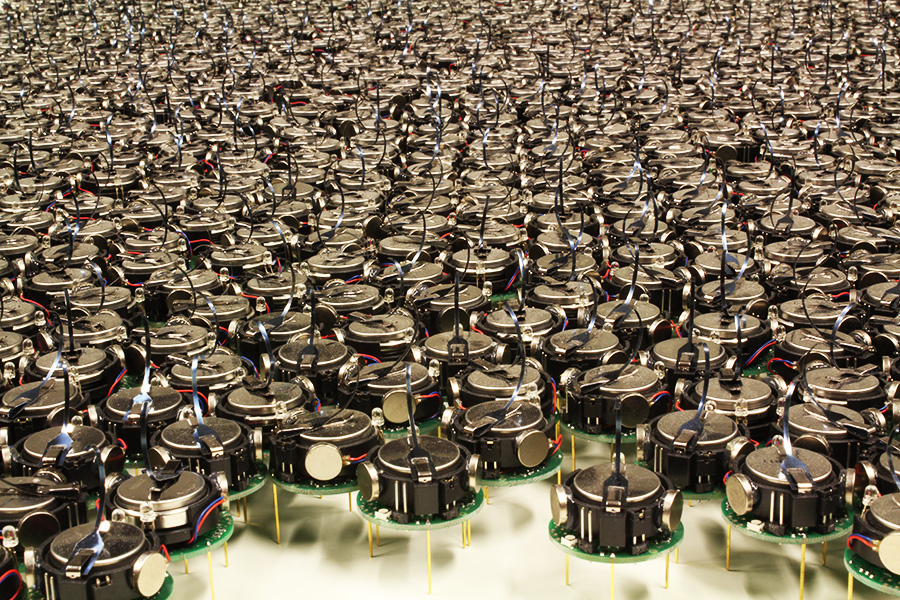
\includegraphics[width=0.28\textwidth]{img/swarms.jpg}
    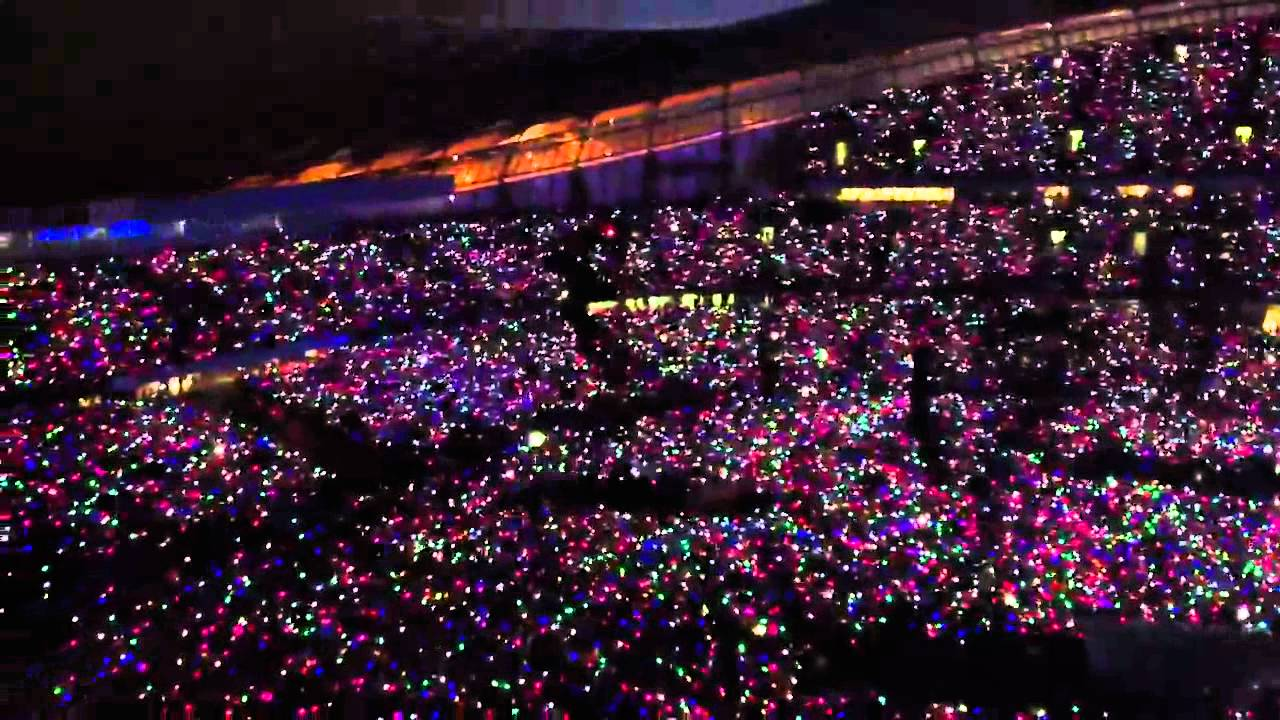
\includegraphics[width=0.333\textwidth]{img/coldplay.jpg}
    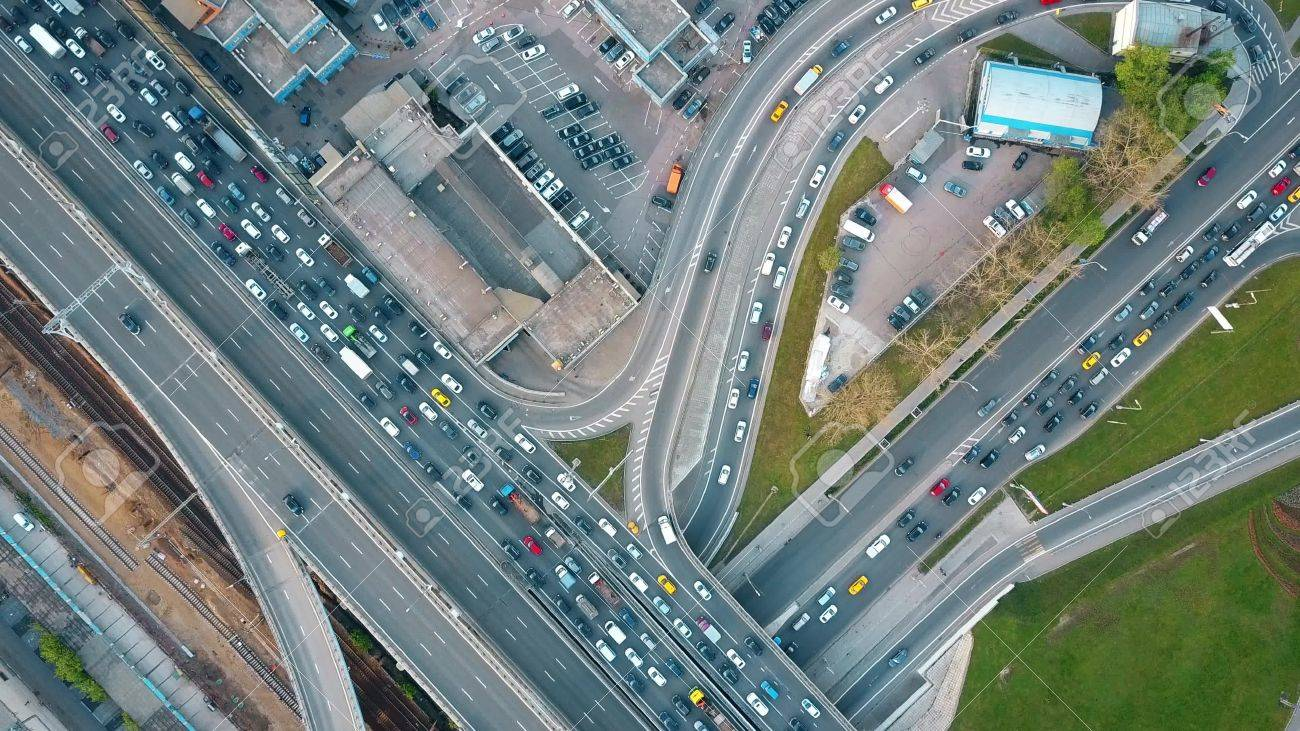
\includegraphics[width=0.333\textwidth]{img/traffic.jpg}	
    \end{center}
  \end{frame}
\begin{frame}{Context -- Cont.}
\begin{alertblock}{Applications}
  \begin{multicols}{3}
    \begin{itemize}
      \item Swarm robotics
      \item Crowd of (augmented) people
      \item Large-scale IoT systems
      \item Smart cities
      \item COMMunity-OrieNted WEARrable Computing Systems (PRIN project)
    \end{itemize}
  \end{multicols}
\end{alertblock}

\begin{block}{Challenges}
  \begin{multicols}{3}
    \begin{itemize}
      \item (Unwanted) Emergents
      \item Local to global mapping
      \item Scale
      \item Failures
      \item Distributed control
      \item Complex \& layered architectures
    \end{itemize}
  \end{multicols}
\end{block}
\centering
\end{frame}
\begin{frame}{Thesis Goal}
  \begin{alertblock}{Thesis goal}
    Finds a \emph{systematic} methodology to \bold{synthesize} and \bold{deploy} \emph{\underline{self-organising}} behaviours of \bold{predictable} outcomes
  \end{alertblock}
  \begin{exampleblock}{Multi-Faceted scientific problem}
    \begin{itemize}
      \item \bold{how} to express collective behaviours (algorithms \& methodologies)
      \item \bold{how} to execute specific behaviours (execution models \& middleware dynamics)
      \item \bold{how} to deploy the computation \emph{\underline{smartly}} (deployment)      
    \end{itemize}
  \end{exampleblock}
\end{frame}
\begin{frame}{State-of-the-art}
  \begin{exampleblock}{Manual design}
  Approaches in which the collective behaviour is \emph{\underline{manually}} designed
  \begin{itemize}
    \item Finite state machines, rule-based systems, etc
    \begin{itemize}
      \item bottom-up, high knowledge requirements and the collective behaviour come up by \emph{\underline{emergence}}
    \end{itemize}
    \item Programming languages with primitives and \emph{collective} abstractions for CPSW (macroprogramming)
    \begin{itemize}
      \item Buzz: a language for programming swarms of drones
      \item \bold{Aggregate computing}: a language for programming collective behaviours based on computational fields
    \end{itemize}
  \end{itemize}  
  
  \end{exampleblock}
  \begin{exampleblock}{Automatic design}
    \begin{itemize}
      \item Genetic algorithms, evolutionary strategies, etc
      \begin{itemize}
        \item \emph{\underline{Black-box}} approach, not predictable, hard to scale-up in complexity.
      \end{itemize}
      \item Single-agent machine learning (e.g., reinforcement learning)
      \begin{itemize}
        \item \emph{\underline{Single-agent}} not suitable for collective behaviours (i.e., uncontrolled emergents)
      \end{itemize}
      \item \bold{Many-agent reinforcement learning}: a way to learn collective behaviours with a large population of agents
    \end{itemize}
  \end{exampleblock}
\end{frame}
\begin{frame}[plain]
\begin{center}
\Huge{\bold{Aggregate Computing}}
\end{center}
\centering
\large{Program the aggregate, not the individual}
\\ \vspace{0.5cm}
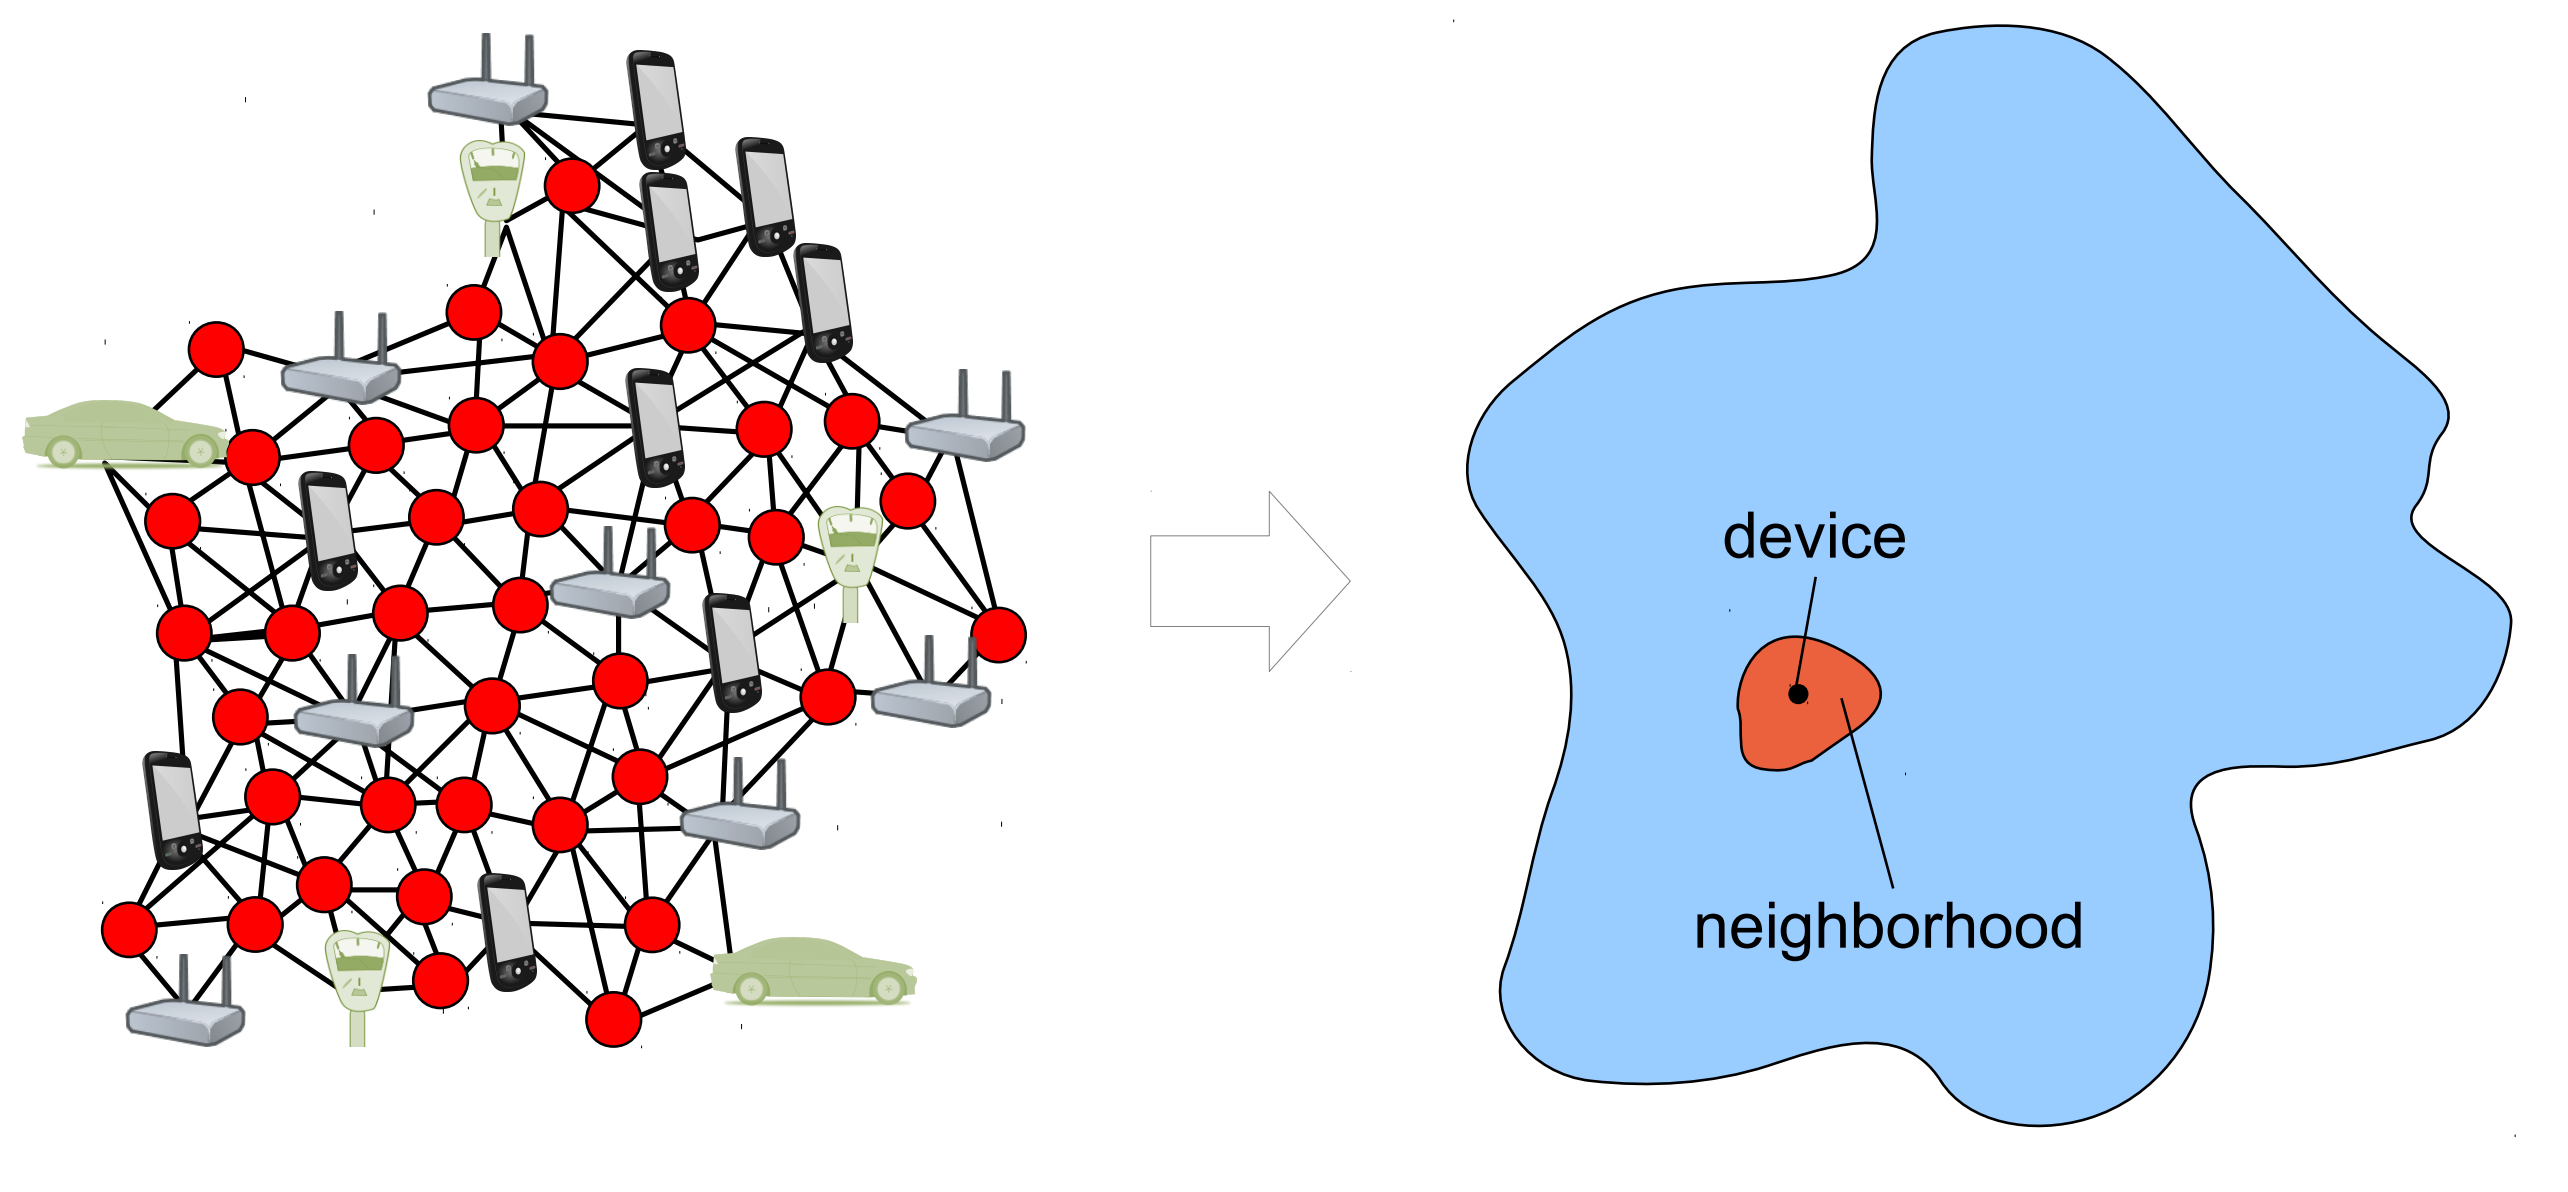
\includegraphics[width=0.8\textwidth]{img/ac.png}
\end{frame}
\begin{frame}{Aggregate Computing -- Foundational and Programming Model}
\begin{block}{Computational Fields}
  A computational field is conceptually a function from the space of devices to a set of values
  \\[0.1cm]
  \begin{center}
  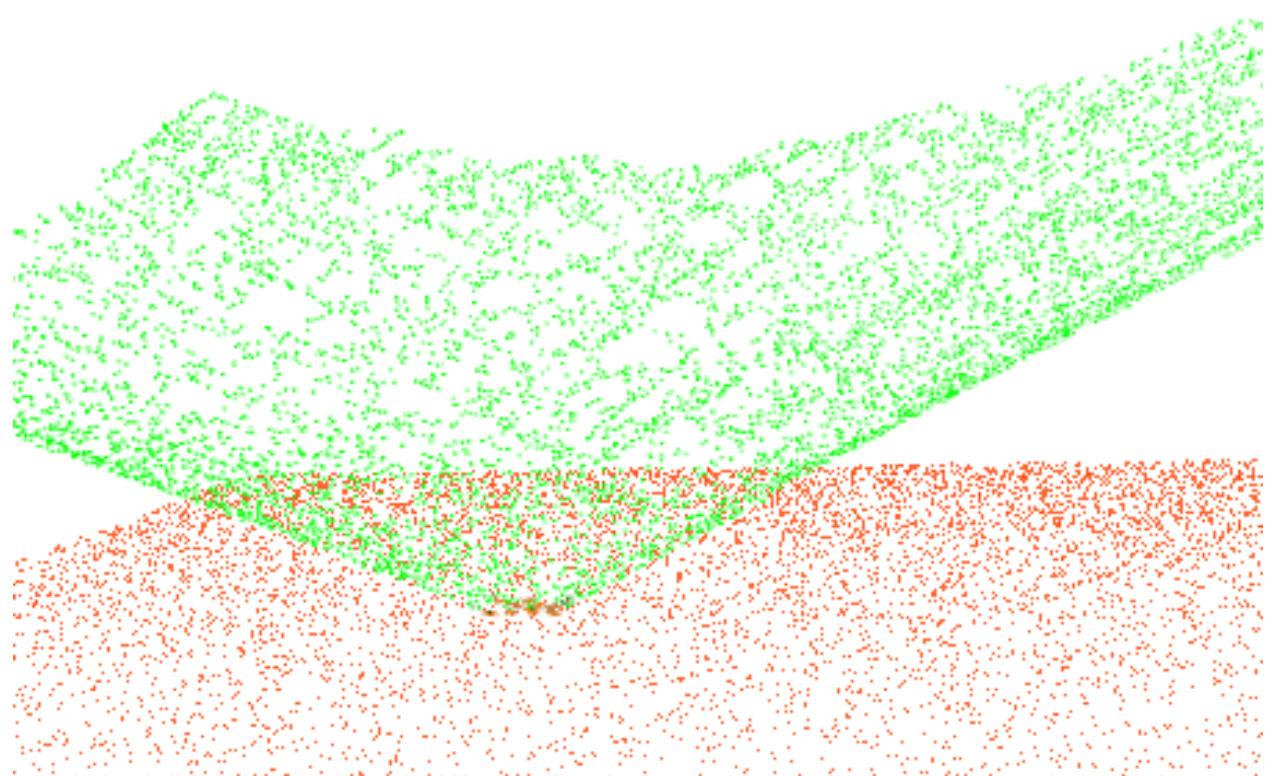
\includegraphics[width=0.3\textwidth]{img/3d-gradient.png}
  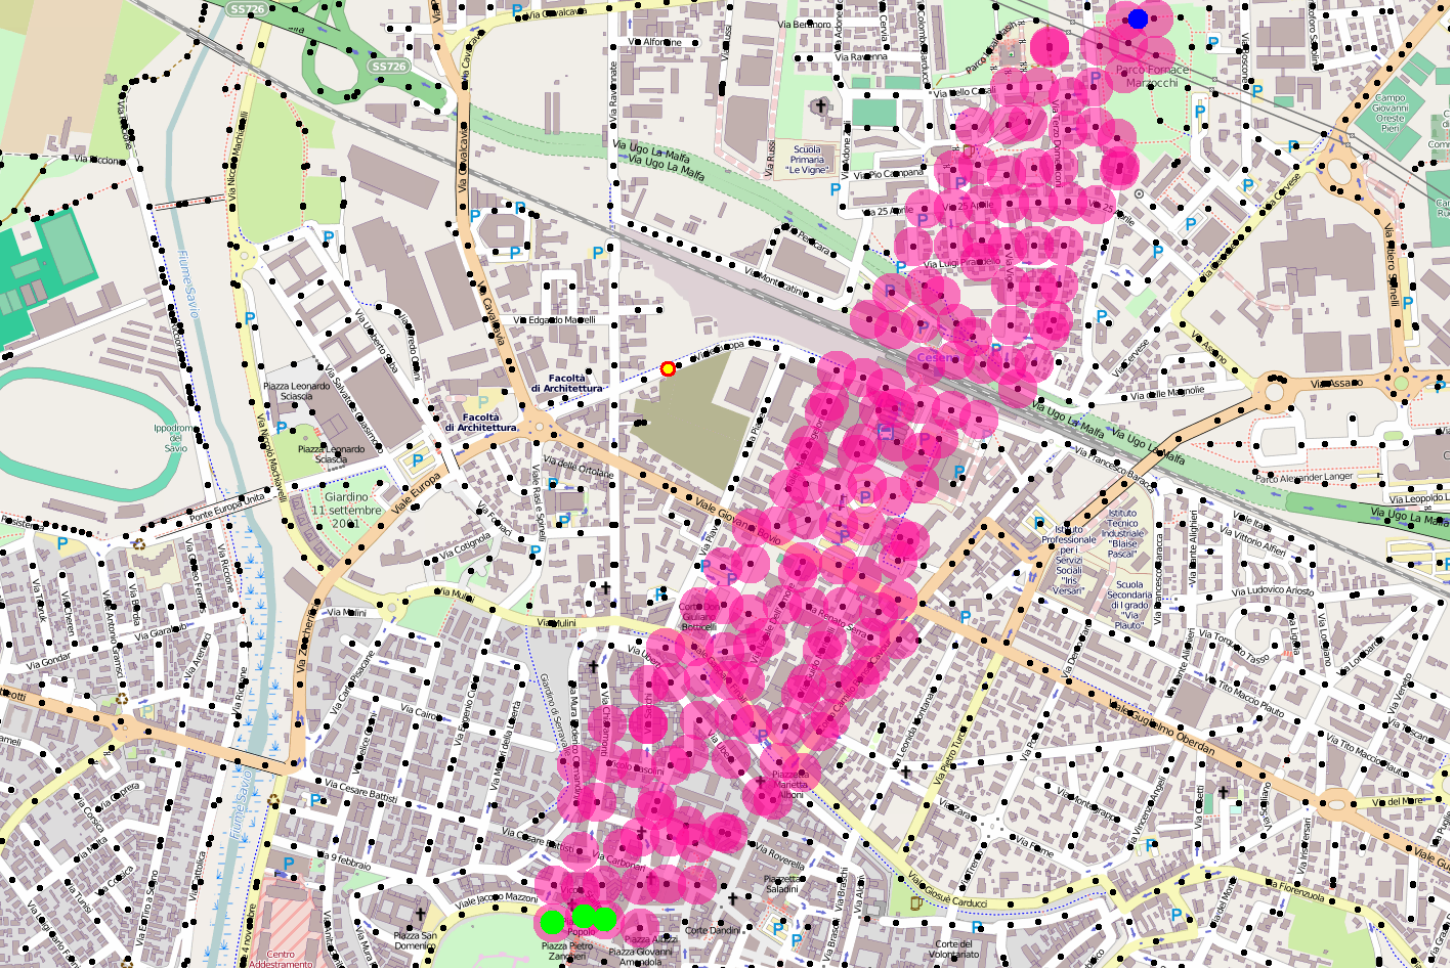
\includegraphics[width=0.28\textwidth]{img/channel.png}
  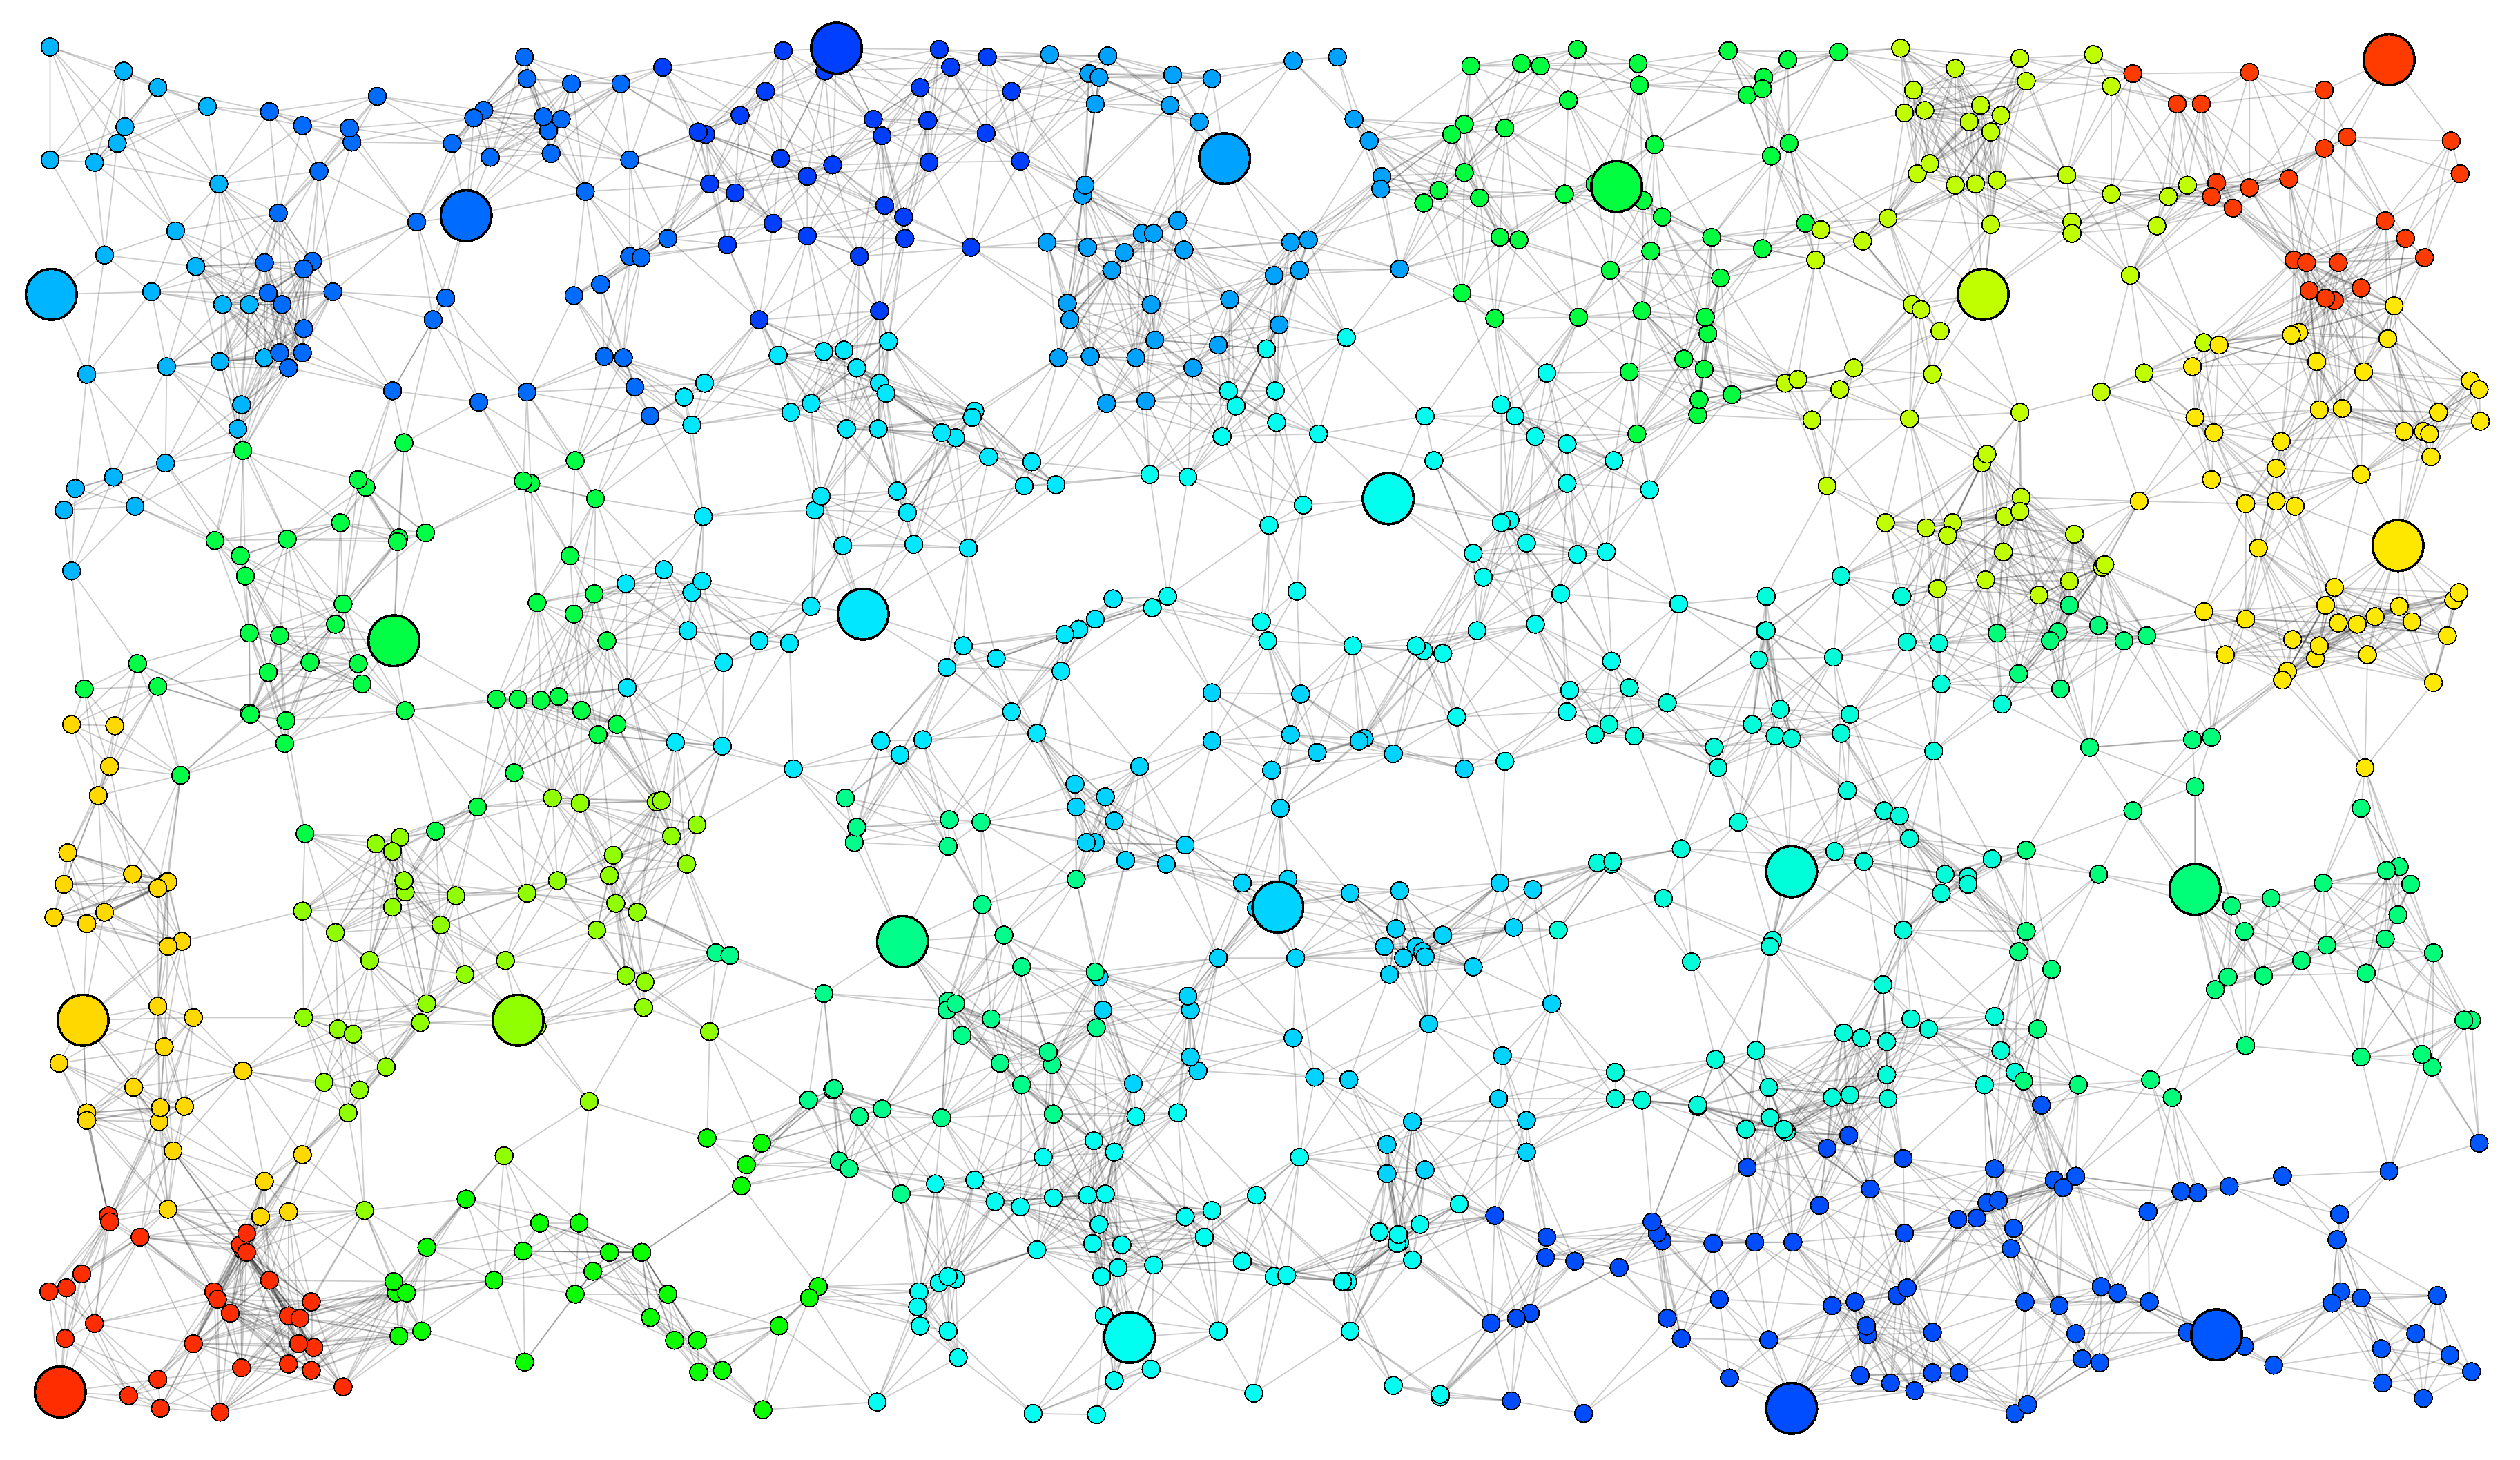
\includegraphics[width=0.3\textwidth]{img/scr-result.png}
  \end{center}
\end{block}
\begin{alertblock}{Field Calculus}
  A language for programming computational fields.
  
  \bold{Primitives}:
  \begin{itemize}
    \item \emph{\underline{neighbours interaction}}: a way to express the interaction with the neighbours (\emph{space})
    \item \emph{\underline{field-evolution}}: a way to express the evolution of the field in \emph{time}
    \item \emph{\underline{space-partition}}: a way to express the space partitioning 
  \end{itemize}
\end{alertblock}  
\end{frame}
\begin{frame}[fragile]{Programming Model -- High-level Idea}
  \begin{center}
    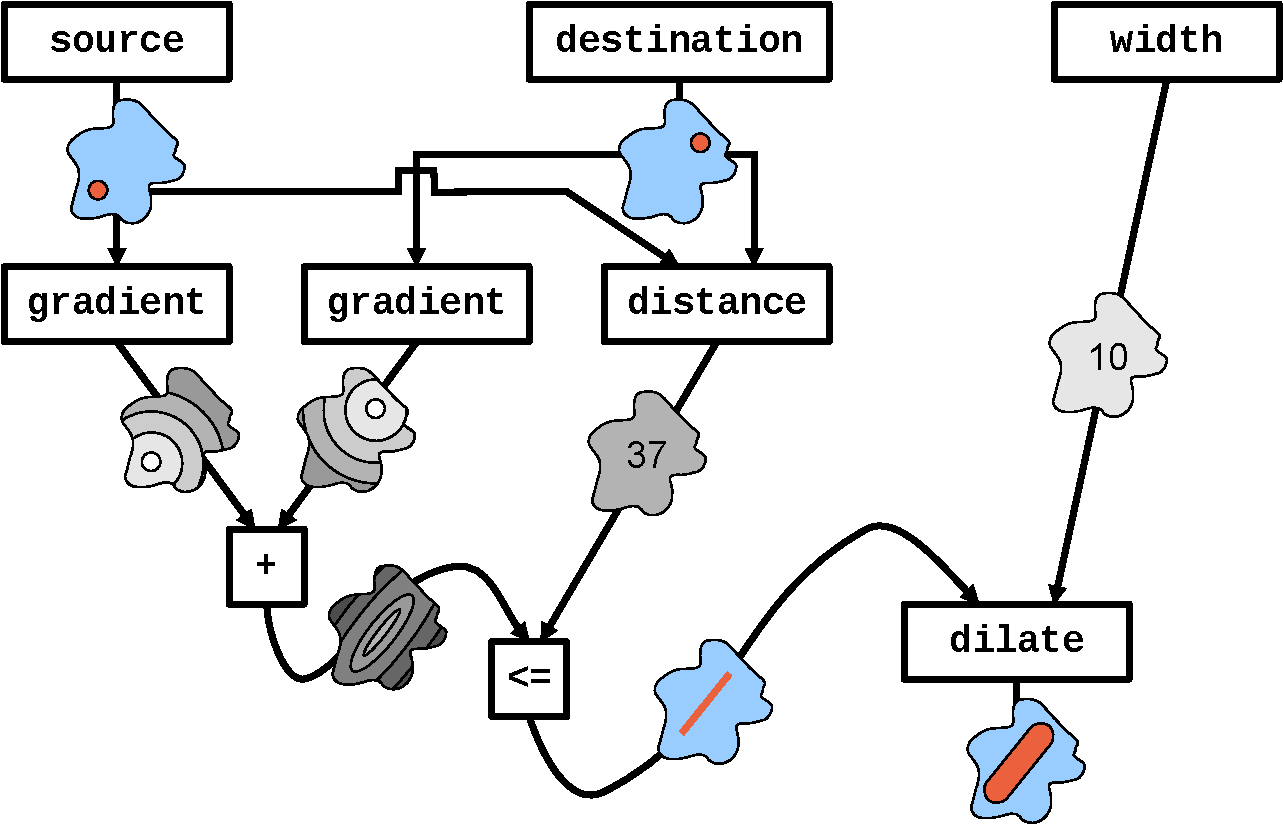
\includegraphics[width=0.48\textwidth]{img/functions.pdf}
    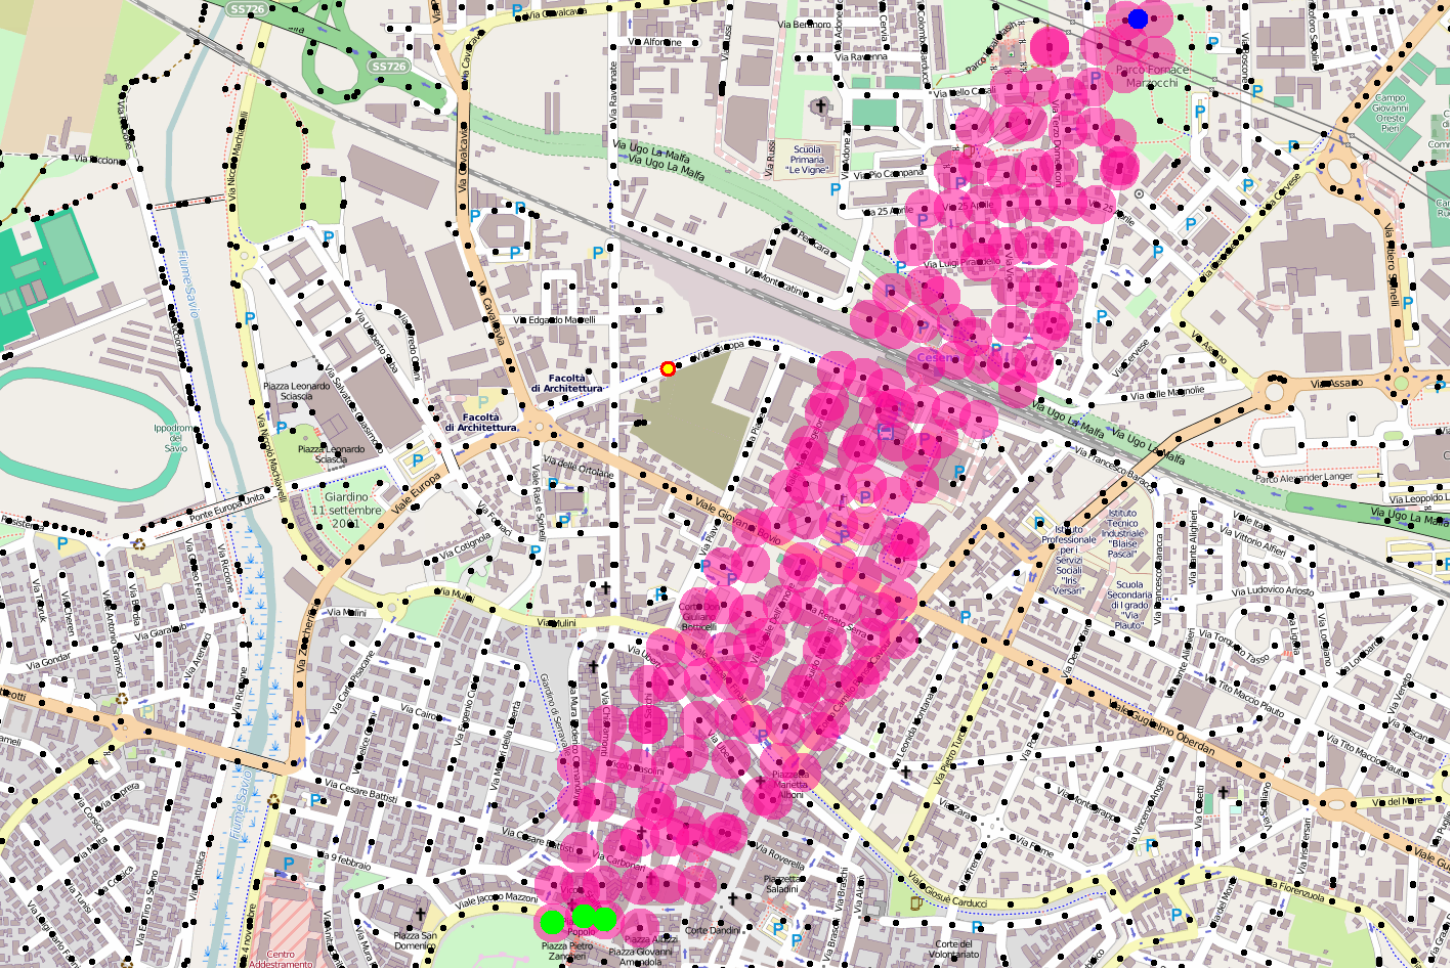
\includegraphics[width=0.48\textwidth]{img/channel.png}
  \end{center}
\begin{minted}{scala}
def channel(source: Boolean, dest: Boolean, width: Double): Double {
  dilate(gradient(source) + gradient(dest) <= distance(source,dest), width)
}
  \end{minted}

\end{frame}
\begin{frame}{Aggregate Computing -- Execution Model \& System Model}
\centering
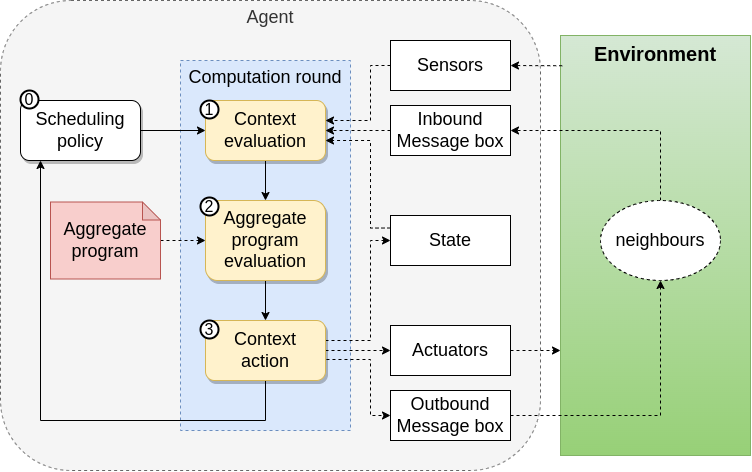
\includegraphics[width=0.8\textwidth]{img/execution-step.png}
\end{frame}
\begin{frame}[plain]
  \begin{center}
\huge{\bold{Many-agent Reinforcement Learning}}
  \end{center}
  \begin{center}
    \large{A multi-agent learning environment in which a \bold{large} group agents learn to \bold{coordinate} their actions to achieve a \emph{\underline{collective}} goal}.
  \end{center}
\end{frame} 

\begin{frame}{Many-agent Reinforcement Learning -- Cont}
\begin{alertblock}{A tentative formal model}
  SwarMDP \faArrowRight \, a formal model composed of a \emph{Swarming agent $\mathbb{A}$} and an \emph{Environment $\mathbb{E}$}.
  \begin{itemize}
    \item The agent $\mathbb{A}$ \faArrowRight \, observation and action spaces, a reward signal and a policy
    \item The environment $\mathbb{E}$ \faArrowRight \, a state space, a population swarming agents, a transition function, a global reward function.
    \item The system evolves in discrete time steps, where the agents $\mathbb{A}$ interact with the environment $\mathbb{E}$ by executing actions and receiving rewards. 
    \item \bold{Goal}: learn a policy $\pi$ that maximises the expected return $\mathbb{E}[\sum_{t=0}^{\infty} \gamma^t R_t]$
  \end{itemize}
\end{alertblock}
\begin{exampleblock}{Challenges \faArrowRight \, Solutions}
  \begin{itemize}
    \item \emph{\underline{Large-Scale}} \faArrowRight \, Homogenous agents (i.e., share the same policy) with \bold{decentralised} execution
    \item \emph{\underline{Partial Observability}} \faArrowRight \, Use \emph{\underline{ neighborhood communication}} to share the information and reaching a collective behaviour through emergence
    \item \emph{\underline{Non-Stationarity}} \faArrowRight \, Use \emph{\underline{centralised}} learning with a global view of the environment
    \item \emph{\underline{Global-Local}} \faArrowRight \, Use both \emph{local} and \emph{global} rewards to learn
  \end{itemize}
\end{exampleblock}

\end{frame}
\begin{frame}{Going towards the state-of-the-art}
  \begin{alertblock}{Engineering Perspective}
    \begin{itemize}
    \item \emph{API Design}: Close the gap between aggregate computing and real-world applications.%, making complex CPS behaviors easier to program.
    \item \emph{Programming Model}: Develop a natural way to express collective behaviors.%, simplifying the development process.
    \item \emph{Intelligent Deployment}: Optimize the deployment of aggregate programs across diverse infrastructures, enhancing adaptability and efficiency.
    \item \emph{Practical Tooling}: Create user-friendly tools for prototyping and deploying aggregate programs, fostering broader adoption.
    \item \textbf{\underline{Key Motivation}}: Aggregate computing requires refined abstractions and tools to effectively engineer the complex world of CPWSs.
    \end{itemize}
    \end{alertblock}
  \begin{alertblock}{Learning Perspective}
      \begin{itemize}
      \item \emph{AC for Learning}: Utilize aggregate computing to build robust and resilient learning infrastructures, e.g., for federated learning.
      \item \emph{Learning for AC}: Leverage machine learning to dynamically optimize and adapt the aggregate computing model itself.
      \item \textbf{\underline{Key Motivation}}: Learning is essential to adapt aggregate computing to the highly dynamic and complex nature of real-world environments.
      \end{itemize}
  \end{alertblock}
\end{frame}
\begin{frame}{Contribution -- One slide}
\centering{\huge{\underline{Languaged-based soft eng} \faArrowRight \, Models, tools, and algorithms are built around a \emph{\underline{programming language}}}}
\\[0.5cm]
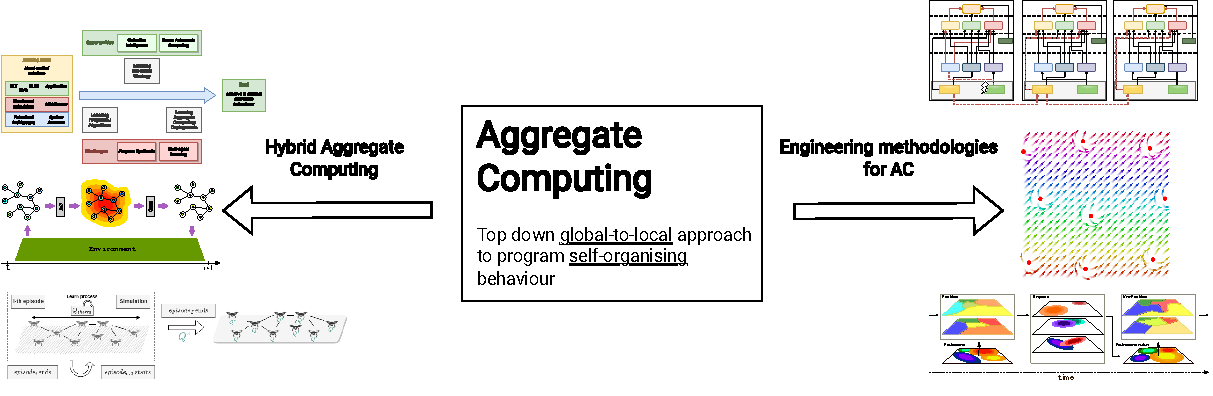
\includegraphics[width=\textwidth]{img/contribution.drawio.pdf}
\end{frame}

\begin{frame}{Hybrid Aggregate computing -- Research Roadmap}
  
  \bold{Highlight goals}:
  \begin{itemize}
    \item \underline{functionality} (e.g., a certain collective behaviour)
    \item \underline{non-functionality} (e.g., energy consumption)
  \end{itemize}
  \bold{and means}:
  \begin{itemize}
    \item \underline{system structures}
    \item \underline{execution strategy}
    \item \underline{algorithms}
  \end{itemize}
  \begin{center}
    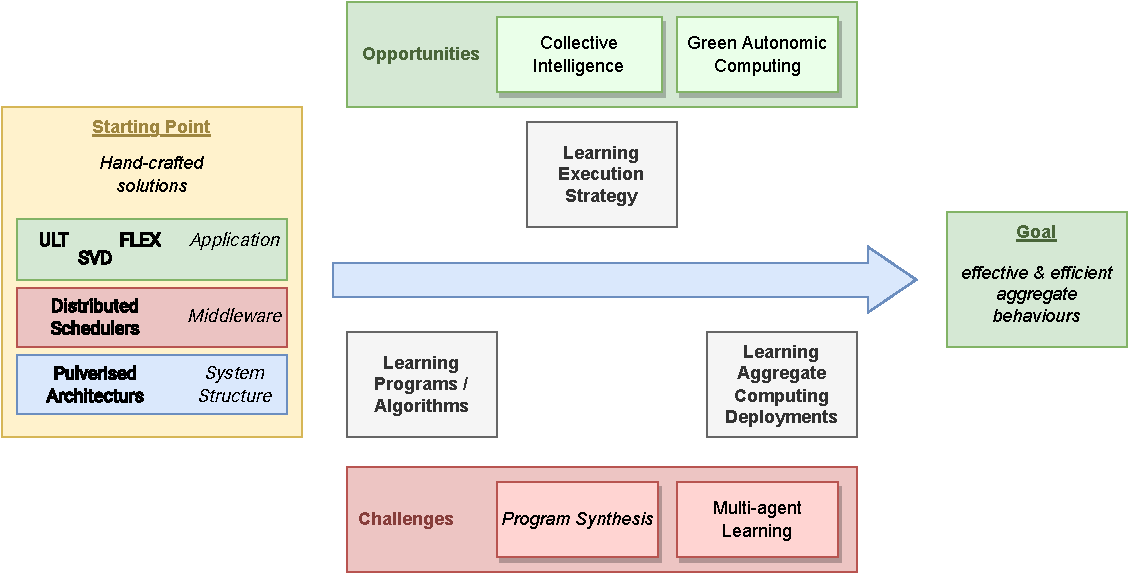
\includegraphics[width=0.6\textwidth]{img/roadmap.pdf}
  \end{center}
\end{frame}
\begin{frame}{Optimizing Execution Policies in Aggregate Computing}

\begin{alertblock}{Problem}
Given the same aggregate program, there exist different execution policies that may prioritize:
\begin{itemize}
\item Convergence Time: Quickly reach a stable global configuration from an initial configuration.
\item Consumption Reduction: Reach the same global configuration while minimizing resource consumption.
\end{itemize}
\end{alertblock}
\begin{alertblock}{Programmatic Solution}
\begin{itemize}
\item Programmable Schedulers: Allow modifying collective scheduling dynamics based on the obtained results.
\item Limitation: These schedulers are static and do not adapt to changes in the environment.
\end{itemize}
\end{alertblock}
\end{frame}

\begin{frame}{Machine Learning for Optimization}
\begin{alertblock}{Idea}
Use machine learning techniques (Q-learning) to learn adaptive and optimized schedulers.
\end{alertblock}
\begin{center}
  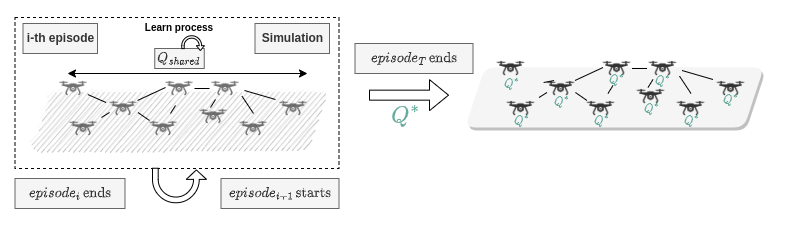
\includegraphics[width=0.9\textwidth]{img/algorithm-learning.png}
\end{center}
\begin{alertblock}{Approach}
\begin{itemize}
\item Q-learning with shared experience: a method for learning in CPSW systems.
\item Goal: Reduce the consumption of \emph{self-stabilizing} collective computations.
\item State: Result of aggregate computation in a fixed time window.
\item Reward: Based on the goal, it rewards convergence or energy consumption, guiding the learning towards the optimal policy.
\end{itemize}
\end{alertblock}
\end{frame}
%\begin{frame}{Hybrid Aggregate Computing -- Execution Strategy}
%  \begin{exampleblock}{Distributed schedulers~\cite{DBLP:conf/acsos/AguzziCV22}}
%    \begin{itemize}
%      \item The aggregete computing model does not \underline{enforce} a global-synchronization
%      \item \emph{\underline{Distributed}} schedulers: \emph{\underline{local}} decisions on the \emph{\underline%{rounds}} of the aggregate program
%      \item Idea: \emph{\underline{learning}} the \emph{\underline{best}} scheduling strategy directly by-doing
%    \end{itemize}
%    \begin{center}
%    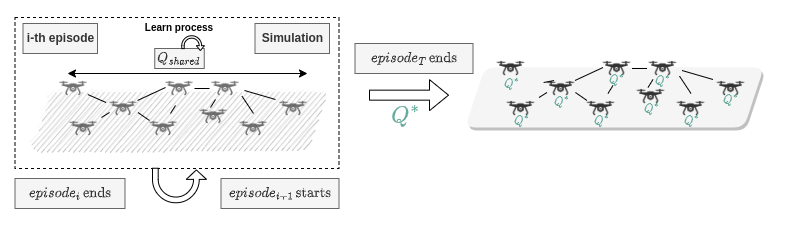
\includegraphics[width=0.9\textwidth]{img/algorithm-learning.png}
%    \end{center}
%  \end{exampleblock}
%\end{frame}
\begin{frame}{Hybrid Aggregate computing -- Algorithms}
  \begin{exampleblock}{Collective Program Sketching~\cite{DBLP:conf/coordination/AguzziCV22}}
    \begin{itemize}
      \item \emph{\underline{holes}}: \emph{\underline{blocks}} of the aggregate program depending on \emph{\underline{environment dynamics}}
      \item \emph{\underline{sketching}}: \emph{\underline{partial}} specification of the aggregate program
      \item Idea: \emph{\underline{synthesis}} of the \emph{\underline{holes}} by \emph{\underline{learning}} from the \emph{\underline{realistic simulation}}
    \end{itemize}
    \begin{center}
    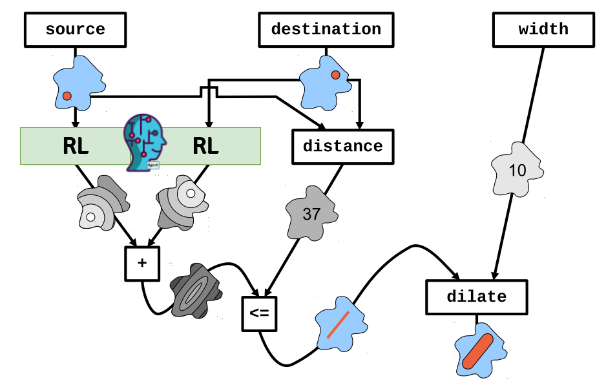
\includegraphics[width=0.5\textwidth]{img/synthesis-3.png}
    \end{center}
  \end{exampleblock}
\end{frame}
\begin{frame}{Hybrid Aggregate computing -- Algorithms}
  
\begin{exampleblock}{Field-Informed reinforcement learning~\cite{acgnn}}
  \begin{itemize}
    \item Aggregate computing is used to \emph{\underline{inform}} the learning process
    \begin{itemize}
      \item Speeding up the training \& Reducing the search space
    \end{itemize} 
    \item Field used as a way to produce a stygmertic representation of the environment
    \item Learning performed through \emph{\underline{deep reinforcement learning}}
    \item Graph-neural networks used as a policy function approximator
  \end{itemize}
\centering
  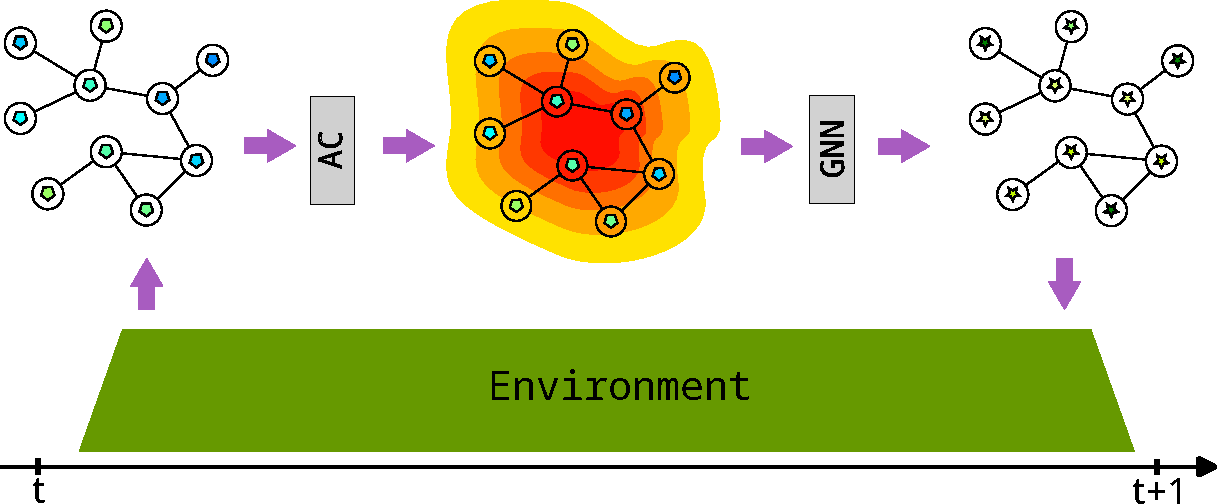
\includegraphics[width=0.6\textwidth]{img/architecture.pdf}
\end{exampleblock}
\end{frame}
\begin{frame}{Hybrid Aggregate computing -- Algorithms}
  
  \begin{exampleblock}{Field-Informed reinforcement learning~\cite{acgnn}}
    Qui continua facendo vedere l'algoritmo
  \end{exampleblock}
  \end{frame}
\begin{frame}{Engineering Methodologies}
\begin{exampleblock}{FRASP~\cite{frasp}}
  
  Functional reactive approach to \emph{\underline{self-organisation}} programming
\begin{itemize}
  \item Inspired by \emph{\underline{functional reactive programming}}, but \emph{\underline{distributed}}
  \item Implementation in a Scala DSL
\end{itemize}
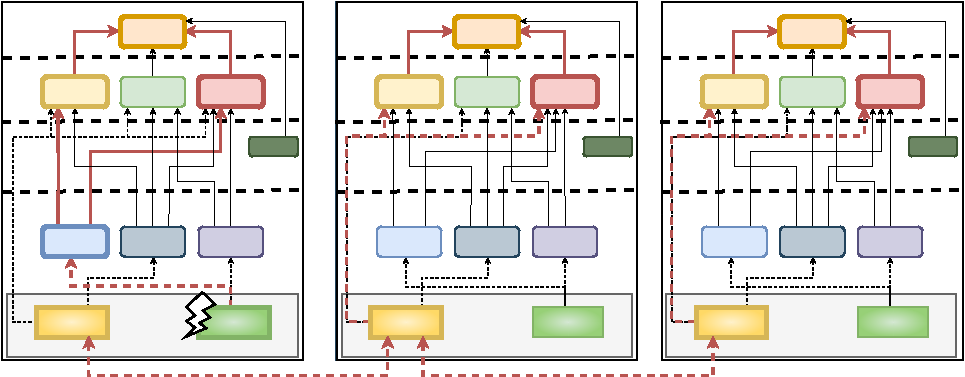
\includegraphics[width=\textwidth]{img/interactions.pdf}
\end{exampleblock}
\end{frame}
\begin{frame}{Engineering Methodologies}
\begin{exampleblock}{MacroSwarm~\cite{macroswarm}}
  \begin{itemize}
    \item An API for expressing \underline{\emph{swarm}} behaviours
    \item \emph{\underline{Composable}}: behaviours can be composed together
    \item \emph{\underline{Extensive}}: cover a wide range of swarm behaviours (e.g., aggregation, flocking, ...)
  \end{itemize}
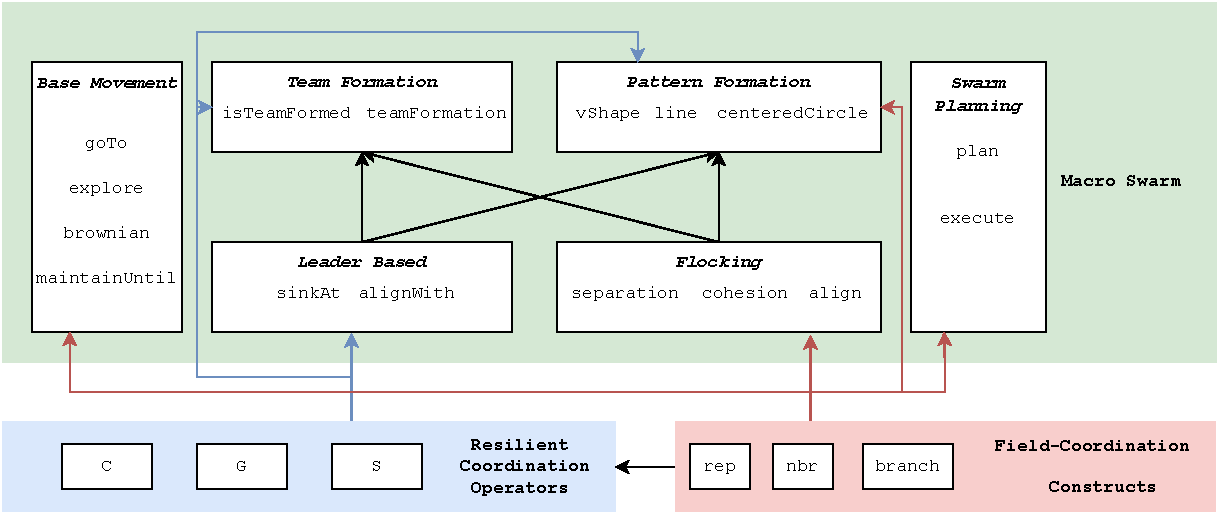
\includegraphics[width=\textwidth]{img/architecture-macro.drawio.pdf}
\end{exampleblock}
\end{frame}
\begin{frame}{Engineering Methodologies -- Cont.}
  \begin{itemize}
    \item \emph{\underline{Swarm Sensing API}}~\cite{swarm-clustering}: \emph{\underline{distributed}} and \emph{\underline{fault-tollerent}} sensing
    \item \emph{\underline{Dev Ops for CPSW}}~\cite{casadei2022towards}: \emph{\underline{continuous integration}} of the \emph{\underline{software}} and the \emph{\underline{physical}} parts of the system
    \item \emph{\underline{High-level abstractions for Distributed sensing}}~\cite{aguzzi2022dynamic}: \emph{\underline{distributed}} and \emph{\underline{fault-tollerent}} sensing
    \item \emph{\underline{Pulverisation architecture}}~\cite{aguzzi2021towards}: A \emph{\underline{opportunistic}} model to \emph{\underline{deploy}} aggregate programs
  \end{itemize}
  \vspace{0.5cm}
  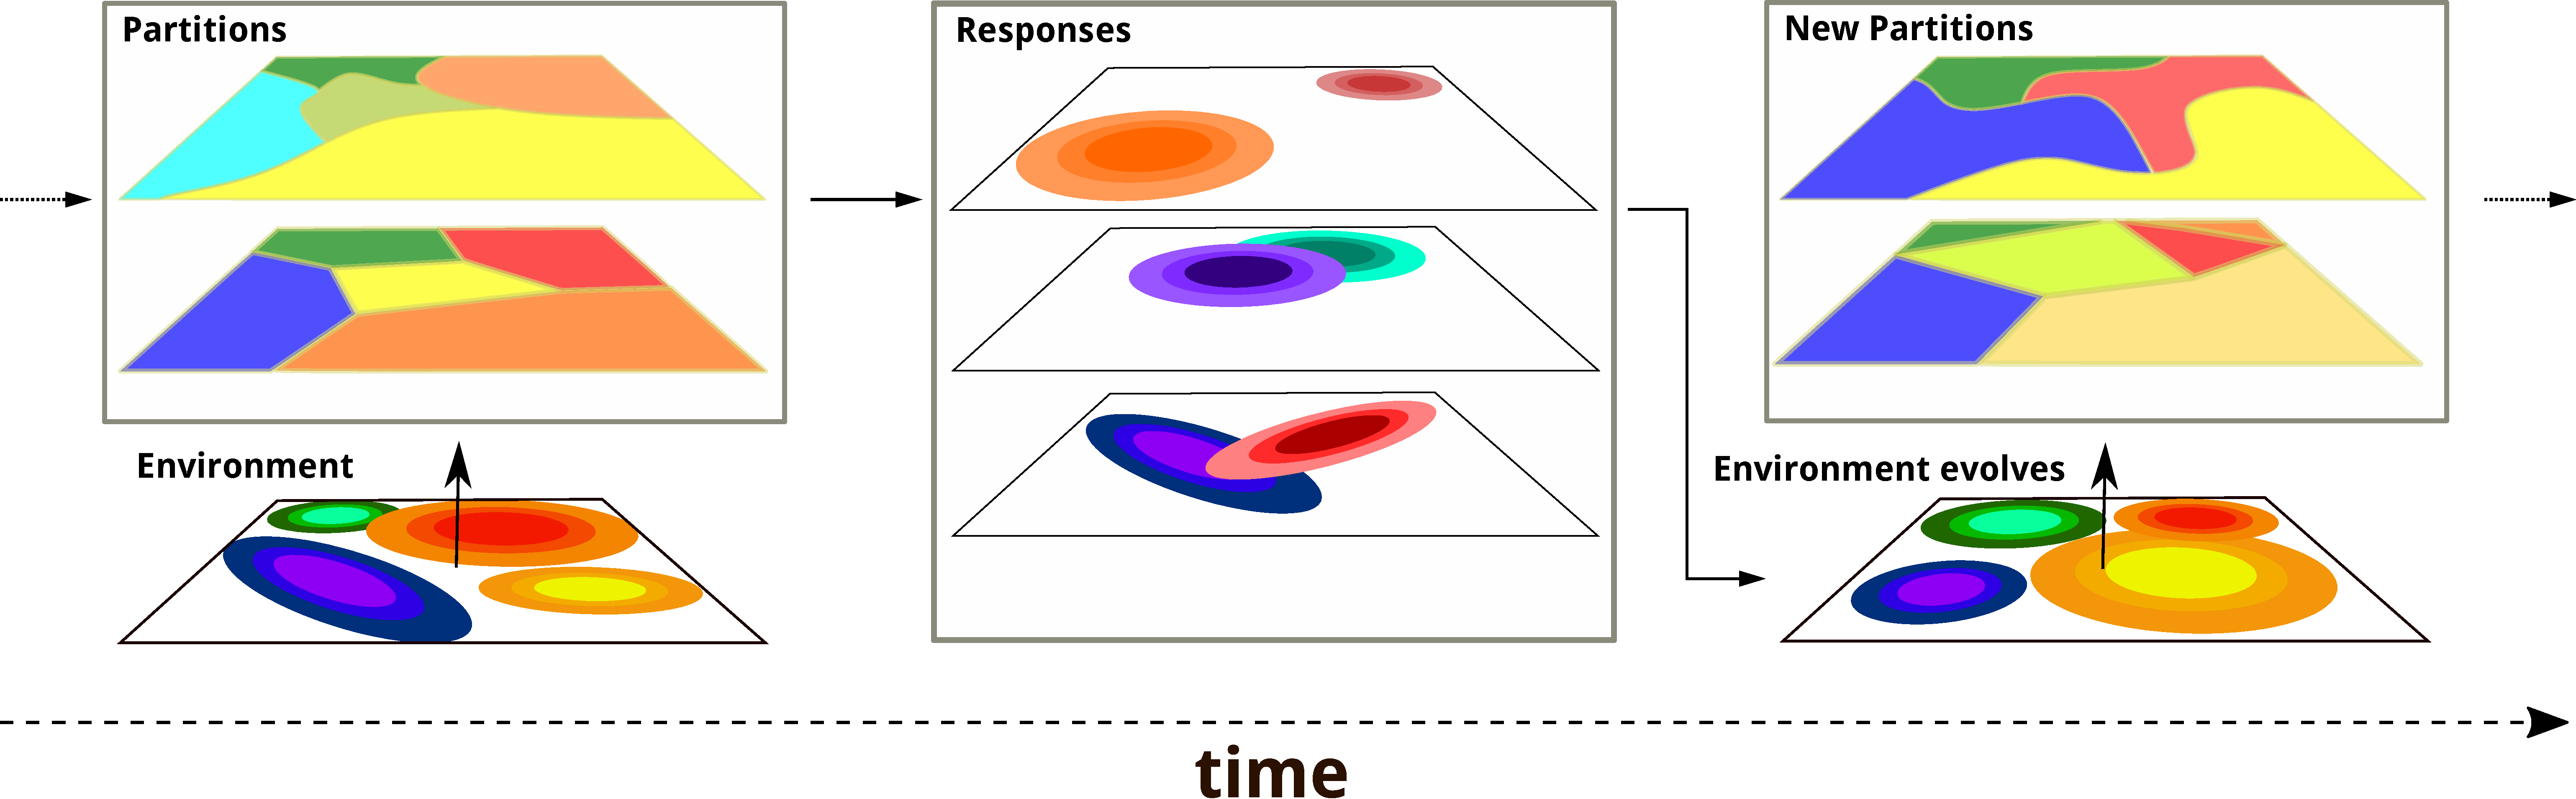
\includegraphics[width=0.45\textwidth]{img/action-with-multilayer.pdf}
  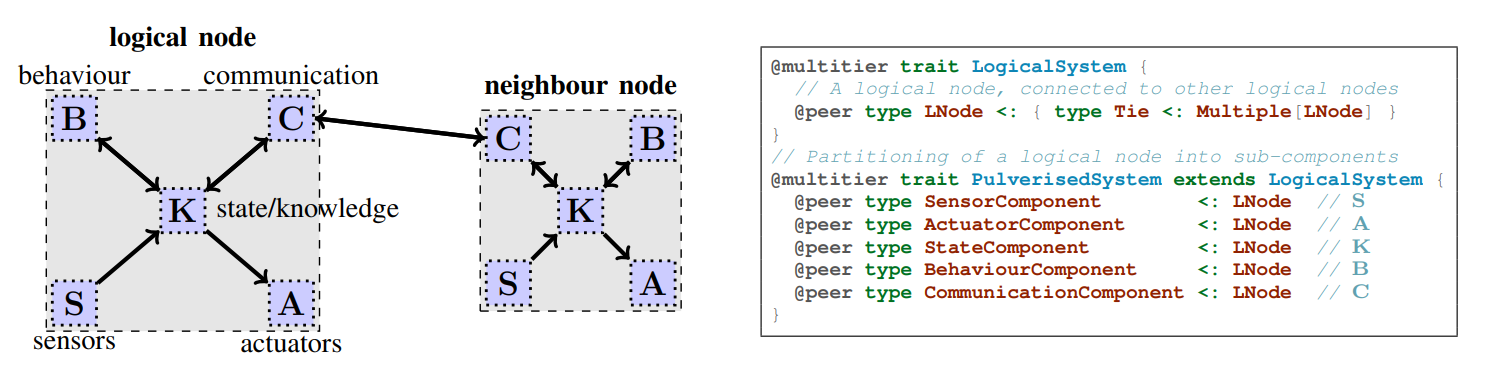
\includegraphics[width=0.53\textwidth]{img/screenshot.png}
  
\end{frame}
\begin{frame}{Tools}
  \vspace{-0.5cm}
  \begin{columns}[t]
    \begin{column}{0.48\textwidth}
      \begin{exampleblock}{ScaRLib~\cite{domini2023scarlib}}
        \footnotesize{
        \begin{itemize}
          \item A tool for cooperative many agent reinforcement learning
          \item Support different learning scheme (centralised, decentralised, mixed)
          \item Binding with state-of-the-art reinforcement learning libraries (e.g., \emph{\underline{PyTorch}})
        \end{itemize}}
        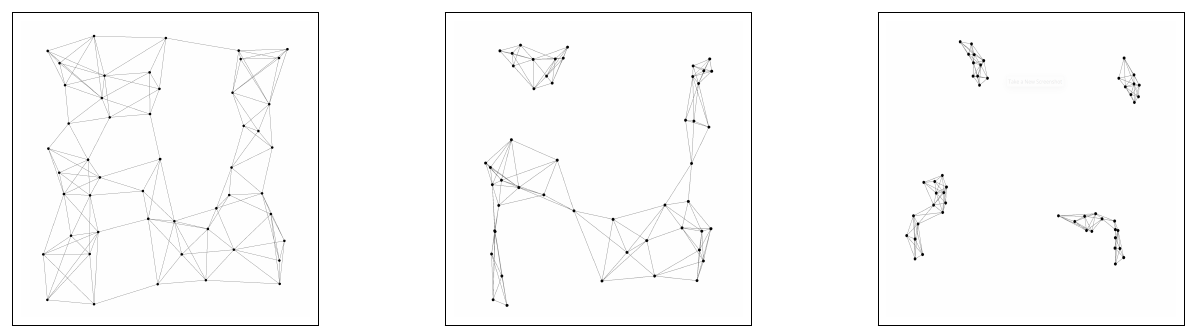
\includegraphics[width=\textwidth]{img/flock.png}
      \end{exampleblock}
    \end{column}
    \begin{column}{0.48\textwidth}
      \begin{exampleblock}{ScaFi-Web~\cite{aguzzi2021scafi}}
        \footnotesize{
        \begin{itemize}
          \item A \emph{\underline{web-based}} simulator for aggregate computing
          \item Useful for \emph{\underline{teaching}} and \emph{\underline{prototyping}}
        \end{itemize}}
        \centering
        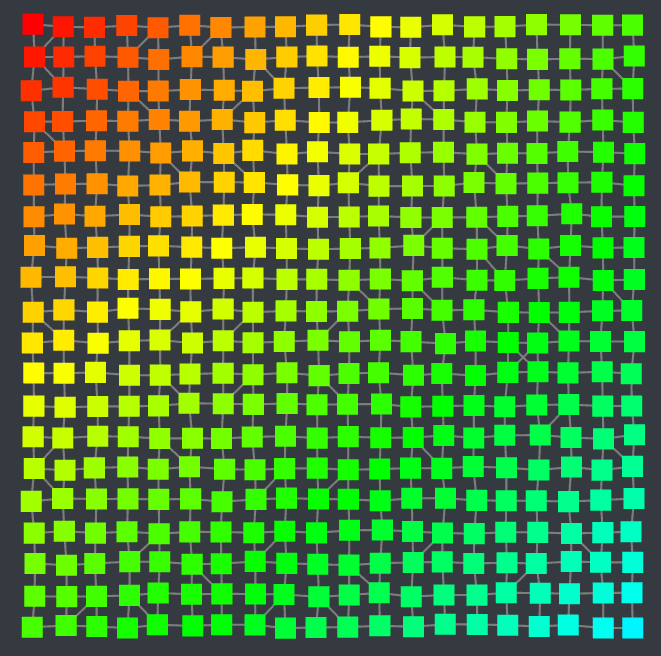
\includegraphics[width=0.5\textwidth]{img/gradient-scafi.png}
      \end{exampleblock}
    \end{column}
  \end{columns}
\end{frame}

\begin{frame}{Conclusion and Future Works}
\begin{itemize}
  \item This thesis is a \emph{\underline{systematic}} approach to the engineering of CPSW
  \item We poses the basis for a \emph{\underline{language-based}} approach to CPSW, putting together:
  \begin{itemize}
    \item \emph{\underline{Learning}}: Field-informed reinforcement learning, collective program sketching, distributed schedulers
    \item \emph{\underline{Tools}}: ScaFi, ScaRLib, ScaFi-Web
    \item \emph{\underline{Methodologies}}: FRASP, MacroSwarm, Swarm-Sensing API
  \end{itemize}
  \item Future works:
  \begin{itemize}
    \item Close the reality gap: deploy the aggregate programs on real CPSW, improve the toolchain, leverage realistic simulators (Gazebo, etc)
    \item Improve the learning algorithms: learn to deploy, learn to adjust runtime execution, etc
    \item AC for learning: aggregate computing as a way create resilient infrastructure for learning (e.g., federated learning)
  \end{itemize}
\end{itemize}
\end{frame}

\begin{frame}
\centering{
  \Huge{Thank you!}
}
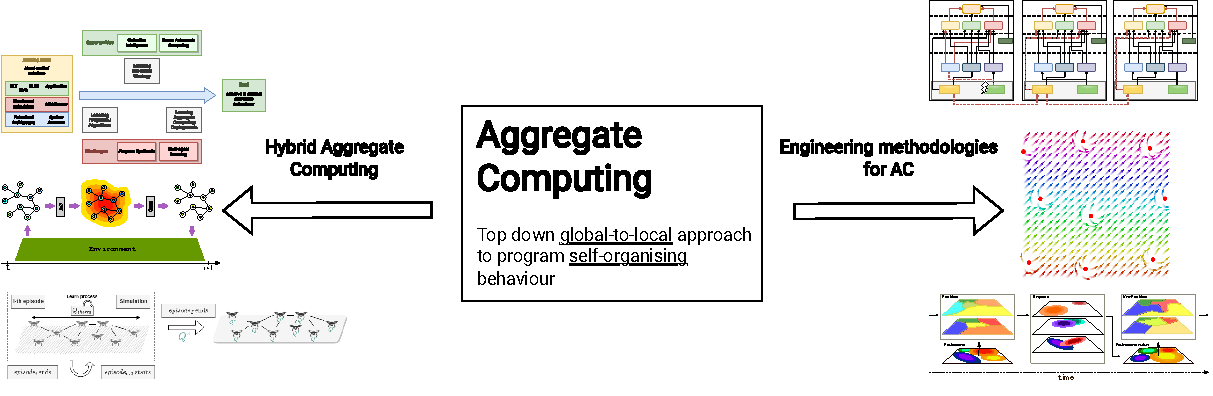
\includegraphics[width=\textwidth]{img/contribution.drawio.pdf}
\end{frame}
\begin{frame}[allowframebreaks]{References}
  \def\bibfont{\footnotesize}
  \printbibliography
\end{frame}

%%%%%%%%%%%%%%%%%%%%%%%%%%%%%%%%%%%%%%%%%%%%%%%%%%%%%%%%%%%%%%%%%%%%%%%%%%%%%%%%
\end{document}
%%%%%%%%%%%%%%%%%%%%%%%%%%%%%%%%%%%%%%%%%%%%%%%%%%%%%%%%%%%%%%%%%%%%%%%%%%%%%%%%


\begin{frame}{Aggregate Computing -- One slide}
  \hsplit{

  \begin{block}{\footnotesize Self-org-like computational model}
  \scriptsize
  
  \lbl{interaction:} \emph{repeated} msg exchange with \bo{neighbours}\vspace{0.1cm}
  
  \lbl{behaviour:} \emph{repeated} execution of \enf{async rounds} of \bo{sense -- compute -- (inter)act} \vspace{0.1cm}
  
  
  \lbl{formal model of executions:} event structures \vspace{0.1cm}
  
  %\lbl{semantics:} (1) device; (2) network; (3) global comp.
  \end{block}
  
  %\uncover<3-4>{
  \begin{block}{}
  \scriptsize
  
  \lbl{abstraction:} \bo{computational fields} ($\mathit{dev/evt} \mapsto \mathbb{V}$) \vspace{0.1cm}
  
  \lbl{formal core language:} field calculus~\cite{vbdacp:ac:survey:jlamp}\vspace{0.1cm}
  
  \lbl{paradigm:} \bo{functional, macro-programming} \vspace{0.1cm} %--- supporting compositionality
  
  \centering
  \imgv{0.22}{channel.pdf}
  \end{block}
  
  \tiny \fullcite{vbdacp:ac:survey:jlamp}%\fullcite{beal2015aggregate-programming}
  
  %}
  }{
  
  %\uncover<2-4>{
  \begin{block}{\footnotesize Why?}
    \scriptsize
    
    {\bold{\faThumbsUp}} \, Decouple the collective specification from the IT networks  \vspace{0.1cm}
    
    {\bold{\faThumbsUp}} \, Scale naturally with nodes in the systems  \vspace{0.1cm}
     
    {\bold{\faThumbsUp}} \, High-level abstractions to devise applications
    
    %\lbl{semantics:} (1) device; (2) network; (3) global comp.
  \end{block}
  %}
  
  %\uncover<4-4>{
  \begin{block}{} %{Engineering approach}
  \imgv{0.32}{layerss.pdf}
  \tiny \fullcite{bpv:aggregate:programming}
  \end{block}
  %}
  }
  
\end{frame}


\begin{frame}{Hybrid Aggregate computing}
  \vspace{-0.5cm}
  \begin{columns}[t]
  \begin{column}{0.31\textwidth}
  \begin{exampleblock}{Research roadmap~\cite{DBLP:conf/icdcs/AguzziCV22}}
    \footnotesize{
    Highlights goals:
  \begin{itemize}
    \item \underline{functionality} (e.g., a certain collective behaviour)
    \item \underline{non-functionality} (e.g., energy consumption)
  \end{itemize}}
  and means:
  \begin{itemize}
    \item \underline{algorithms}
    \item \underline{execution strategy}
    \item \underline{system structures}
  \end{itemize}
    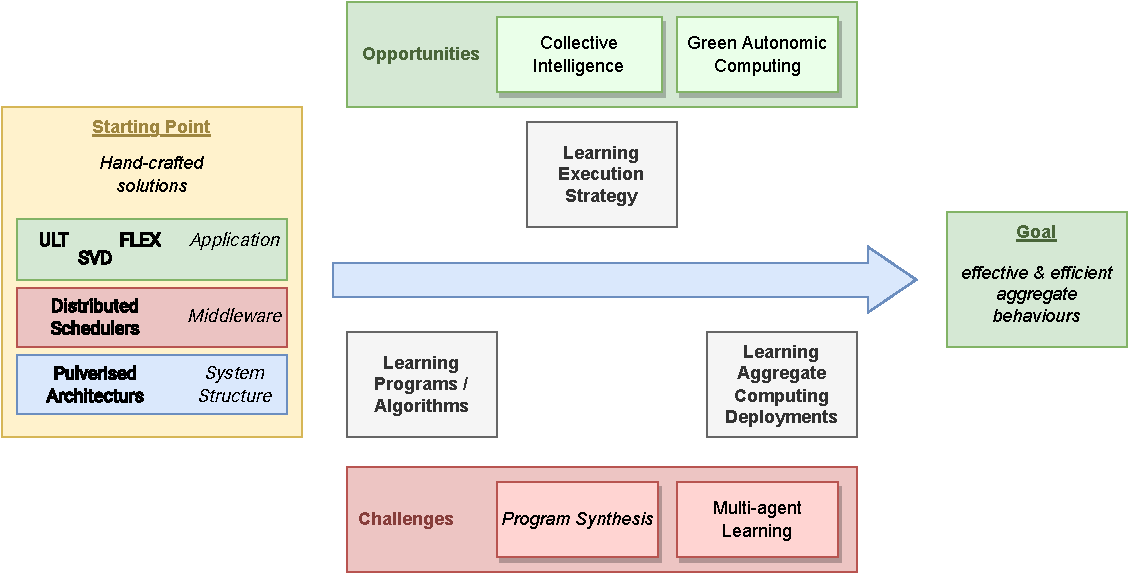
\includegraphics[width=\textwidth]{img/roadmap.pdf}
  \end{exampleblock}
  \end{column}
  
  \begin{column}{0.31\textwidth}
  \begin{exampleblock}{Collective Program Sketching~\cite{DBLP:conf/coordination/AguzziCV22}}
    \footnotesize{
    %% breaks the above sentence in itemize:
    \begin{itemize}
      \item \emph{\underline{holes}}: \emph{\underline{blocks}} of the aggregate program depending on \emph{\underline{environment dynamics}}
      \item \emph{\underline{sketching}}: \emph{\underline{partial}} specification of the aggregate program
      \item Idea: \emph{\underline{synthesis}} of the \emph{\underline{holes}} by \emph{\underline{learning}} from the \emph{\underline{realistic simulation}}
    \end{itemize}}
    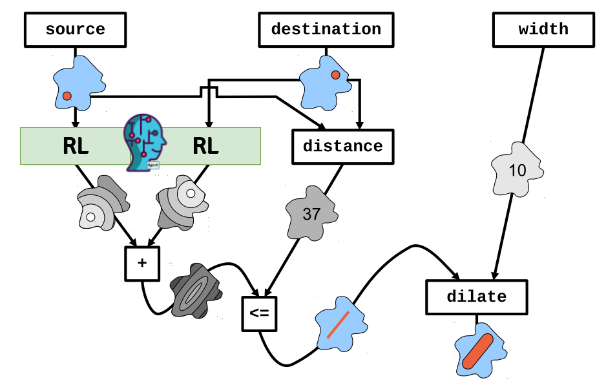
\includegraphics[width=\textwidth]{img/synthesis-3.png}
  \end{exampleblock}
  \end{column}
  \begin{column}{0.31\textwidth}
  \begin{exampleblock}{Distributed schedulers~\cite{DBLP:conf/acsos/AguzziCV22}}
    \footnotesize{
    \begin{itemize}
      \item The aggregete computing model does not \underline{enforce} a global-synchronization
      \item \emph{\underline{Distributed}} schedulers: \emph{\underline{local}} decisions on the \emph{\underline{rounds}} of the aggregate program
      \item Idea: \emph{\underline{learning}} the \emph{\underline{best}} scheduling strategy directly by-doing
    \end{itemize}
    }
    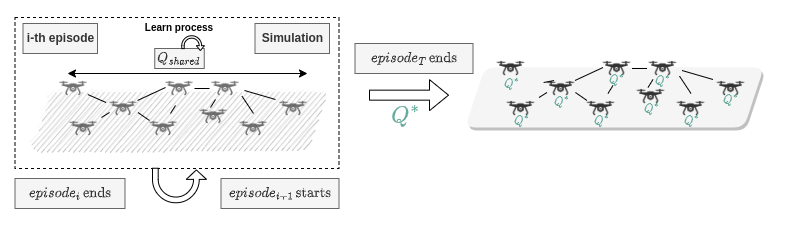
\includegraphics[width=\textwidth]{img/algorithm-learning.png}
  \end{exampleblock}
  \end{column}  
  \end{columns}
  \end{frame}